%!TeX root=MemoriaTFG.tex

\chapter{Simulación de trayectorias}
Definiremos como simulación de una trayectoria al proceso por el cual, mediante los valores 
medibles y cuantificables extraídos del proceso de análisis, se recrea una trayectoria que cumpla 
los mismos criterios. El proceso de simulación (figura )de esta propuesta tiene dos procesos principales.
Primero se generará el camino dada las probabilidades analizadas desde el nodo inicio seleccionado.
Posteriormente se realizará la simulación de la trayectoria por el camino seleccionado.
\begin{figure}[!htb]
\begin{minipage}{0.48\textwidth}
\centering
\includegraphics[width=0.9\textwidth]{./Imagenes/TrackGenerationSegments.png}
\caption{Generación de camino.}
\label{figure:PointToProjection}
\end{minipage}\hfill
\begin{minipage}{0.48\textwidth}
\centering
\includegraphics[width=0.9\textwidth]{./Imagenes/TrackGenerationPoints.png}
\caption{Generación de puntos.}
\label{figure:PointToPoint}
\end{minipage}
\end{figure}

\section{Generación de un camino}

La estructura lógica comentada en la sección \ref{section: EstructuraLogica} nos permite 
almacenar en las aristas la información referente a la frecuencia relativa de paso.
Para generar un camino, se realizará un proceso iterativo por el cual mediante un nodo origen, 
asignado por parámetro de entrada, se seleccionará uno de los caminos, manteniendo la 
distribución probabilística del conjunto de aristas, de forma que si una de las aristas tiene una 
frecuencia del 25\% de las detecciones, con un número suficiente de muestras se cumpliría dicha 
distribución. 
\begin{figure}[!htb]
\begin{center}
\includegraphics[width=0.75\textwidth]{./Imagenes/SimulationProbabilities.png}
\caption{Ejemplo de probabilidades dentro de un nodo intermedio entre rutas.}
\label{fig:PointGeneration02}
\end{center}
\end{figure}

El proceso de selección de aristas continuará hasta que la suma de las distancias 
acumule el total de distancia por recorrer, que será otro de los parámetros de entrada.
La implementación de este proceso se encuentra en el método \textit{create\_path} de la 
implementación del \textbf{\textit{interactor}} \textit{simulate\_track\_impl}

\begin{lstlisting}[caption={Método create\_path}\label{algoritmo:create_path},language=Python] 
    def create_path(self, origin, dist):
        path = []
        distance_created = 0
        prev_node = origin
        path.append(origin)
        while distance_created < dist:
            next_node = self.get_most_frequent_node(prev_node, path)
            distance_aux = distance_created + self.graph.get_edge_by_nodes(prev_node, next_node)['length']
            if distance_aux < dist:
                distance_created = distance_aux
                path.append(next_node)
                prev_node = next_node
            else:
                return path, distance_created
        return path, distance_created
\end{lstlisting}

\section{Generación de los segmentos}

Una vez se tiene seleccionado el camino que se realizará. Se simulará cada uno de los segmentos individualmente.
Para ello se identificara el nodo origen y final del segmento y se generarán todos los puntos necesarios hasta
que la distancia a ese punto sea menor a una $d$, donde $d$ es una distancia parametrizada y modificable. 
La implementación de este proceso se encuentra en el método \textit{simulate\_segment} de la implementación 
del \textbf{\textit{interactor}} \textit{simulate\_track\_impl}

\begin{lstlisting}[caption={Método simulate\_segment}\label{algoritmo:simulateSegment},language=Python] 
    def simulate_segment(self, segment):
        aux = 0
        origin_node = segment[0]
        target_node = segment[1]
        segment = []
        origin_point = TrackPoint(self.graph.get_nodes()[origin_node]['x'], self.graph.get_nodes()[origin_node]['y'])
        target_point = TrackPoint(self.graph.get_nodes()[target_node]['x'], self.graph.get_nodes()[target_node]['y'])
        try:
            dest, aux = self.calculate_point(segment, origin_node, target_node, origin_point, target_point)
            next = dest
            while aux > DISTANCE_TO_FINAL_NODE:
                dest, aux = self.calculate_point(segment, origin_node, target_node, next, target_point)
                next = dest
        except KeyError:
            pass
        return segment
\end{lstlisting}

\newpage
\section{Generación del punto pseudo-aleatorio}

Es en este punto de la lógica donde se realiza la generación de puntos de forma pseudo-aleatoria, 
utilizando información procedente de los análisis realizados.
Para la creación de un punto a partir de otro se necesita una distancia $d$ y un ángulo $\alpha$ como 
se muestra en la figura \ref{fig:PointGeneration01}
\begin{figure}[htb]
\begin{center}
\includegraphics[scale=0.75, width=0.3\textwidth]{./Imagenes/PointGeneration01.png}
\caption{Ejemplo de generación de punto a partir de una distancia $d$ y un ángulo $\alpha$.}
\label{fig:PointGeneration01}
\end{center}
\end{figure}

Cada punto sera generado teniendo en cuenta el punto anterior. Se encontrará la proyección del segmento
más cercano y se centrará el ángulo en el nodo inmediatamente posterior, con una desviación $\beta$ 
parametrizada y modificable. El proceso queda ilustrado en la figura \ref{fig:PointGeneration02}

\begin{figure}[htb]
\begin{center}
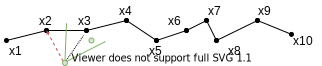
\includegraphics[width=0.75\textwidth]{./Imagenes/PointGeneration02.png}
\caption{Ejemplo de detección de proyección cercana y generación de punto.}
\label{fig:PointGeneration02}
\end{center}
\end{figure}

La distancia para la generación del punto se obtendrá de una elección aleatoria siguiendo un proceso 
llamado \textit{Inverse transform sampling}, por el que se genera un número pseudo-aleatorio a partir 
de una función acumulativa dada una distribución probabilística \cite{Sigman01}.

La distribución probabilística de la distancia punto a punto se obtiene a partir de la información 
que se genera en el proceso de análisis. Se puede ver un ejemplo en la figur 
\ref{figure:PointToPoint} mostrada en la sección \ref{section: AnalisisDistancias}.

\section{Exportación de trayectoria a fichero .\ac{GPX}}
En esta sección se pretende describir la característica del aplicativo para realizar la exportación a GPX.
